
\chapter{From Single Player Games to Two Player Games}

\section{Games under study}

This project focuses on three games: \textit{Five Field Kono}, \textit{Nine Men's Morris} and \textit{ASALTO}.

\bigskip

\subsection{Five Field Kono}

%TODO : describe origin/ rules/ etc...
Five Field Kono is a Korean strategy game. It is played on a $5\times 5$ grid. Its initial configuration is as presented in figure \ref{fig:FFK_initial}. 

\begin{figure}[h]
\centering
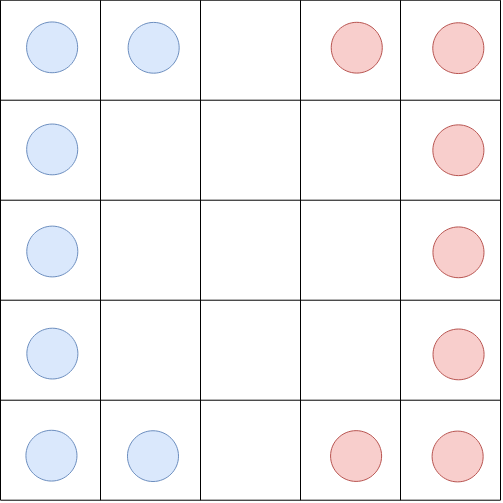
\includegraphics[width = 0.3\hsize]{figures/FFK_rules.png}
\caption{Initial configuration of Five Field Kono. The two players (in blue and red) have seven pawns each.}
\label{fig:FFK_initial}
\end{figure}

The two opponents move one of their pawns in turn knowing that a pawn can only be moved diagonally to an adjacent square (forwards or backwards). A player wins if all his pawns have taken the positions initially held by his opponent's pawns (see figure \ref{fig:FFK_ending}).

\begin{figure}[h]
\centering
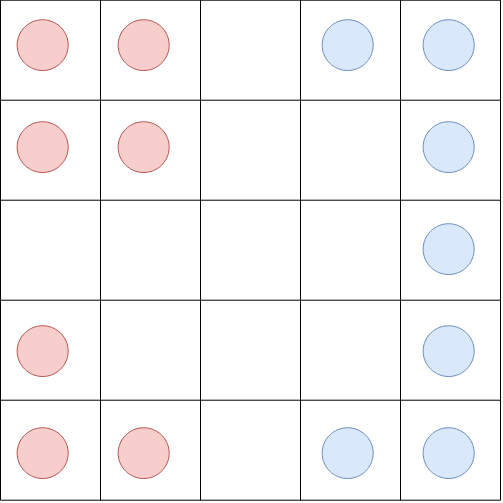
\includegraphics[width = 0.3\hsize]{figures/FFK_ending.png}
\caption{Situation where the blue player wins at Five Field Kono. Every blue pawn is in a square initially occupied by a red pawn (see figure \ref{fig:FFK_initial})}
\label{fig:FFK_ending}
\end{figure}


\subsection{Nine Men's Morris}

Nine Men's Morris is also a Korean strategy game \citep{9MM_rules}. At first the two opponents place in turn their pawns on the board (figure \ref{fig:9MM_initial}). When three pawns are aligned on the board, we say that they form a \textbf{mill}. Each time a player does a mill, he can remove one of his opponent's pawns on the board (that is not already in a mill if possible). Once both players have placed all their pawns, they move in turn one of them to an adjacent empty position. In this second phase, creating a meal has the same effect as before. A player wins if his opponent cannot move or has only two pawns left.

\begin{figure}[h]
\centering
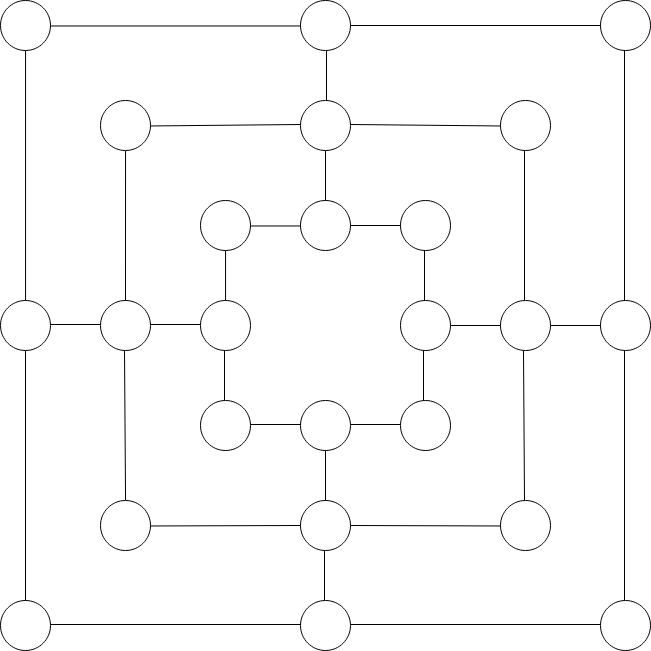
\includegraphics[width = 0.3\hsize]{figures/9MM_initial.png}
\caption{Board for Nine Men's Morris. The circles are the positions where the pawns can be placed or moved. Two positions are adjacent if there is an edge that links them.}
\label{fig:9MM_initial}
\end{figure}


\subsection{ASALTO}

\section{Representing Two-Players games in ASP}

\subsection{Similarities and Differences with Single-Player games}

%TODO source single player game
Representing Two-Players games in ASP follows the same scheme as for Single-Player games \cite{thielscher2009answer}. However, the predicate \texttt{role/1} needs to be modified to include the \textit{color} of each player. And the predicate \texttt{legal/3} has to take into account the fact that this is a turn-based game: a player has the right to play if and only if it is his turn.

\bigskip

Also, we will consider that each \textit{cell} has a set of coordinates (represented by the function \texttt{coord}), and a \textit{state}. For example, if the red player has a red pawn on the cell of coordinates $(1,3)$ at time $4$, then its translation in ASP is: \texttt{holds(cell(coord(1,3),red),4).}

\bigskip

For the moment, we only have studied single-phase game (in the background chapter, and in \cite{thielscher2009answer}). But \textit{Nine Men's Morris} and \textit{ASALTO} are two-phases games: in both of them, players place their pawns before moving them. So we need to define a new predicate \texttt{phase/2} that will appear in the bodies of the rules that define \texttt{legal/3}

\subsubsection{How to describe a two-players-game in ASP}

\begin{enumerate}

\item First, we describe the two players, by using \texttt{role/2}, that takes the name of the player as first argument, and his color for its second argument. From now on, we will suppose the two players are respectively called \textit{player1} and \textit{player2}.  

\item Also, we add the following rule: \newline
\texttt{opponent(P1, P2) :- role(P1, C1), role(P2, C2), P1 != P2.}

\item Then we describe the game as if it was a single player game with only one phase \citep{thielscher2009answer} (we forget that this is a turn based game with one or more phases). In particular, we will have to define the predicates \texttt{holds/3}, \texttt{legal/3}, \texttt{terminal/1}, and \texttt{wins/2}. Moreover,  \texttt{legal(P,M,T)} should only rely on \texttt{holds(C,T)} (at time T \textit{only}), \texttt{role/2}, and \texttt{opponent/2} for the moment. That way, \texttt{legal/3} does not depend on the previous actions or on the previous states, but only on the current states of the game.

\item In each rule that defines \texttt{legal/3} (of the form \texttt{legal(Player, a(X), T)}), we add the following predicate in the body: \texttt{can\_play(Player, a, T)}. This predicate is true if an only if \texttt{Player} has the right to perform an action of type \texttt{a} at time \texttt{T}. 

\item We define the predicate \texttt{can\_play/3}. For instance, in the case of the single-phase turn-based game, \texttt{can\_play/3} can be defined in the following way:\newline
\texttt{turn(player1, 1). }\\
\texttt{turn(P1, T+1) :- time(T), turn(P2, T), opponent(P1, P2).}\\
\texttt{can\_play(Player, Action, T) :- turn(Player, T).}


\item If the game has more than one phase, we need to describe the mechanism of the phase. At time $T=1$, we are in the first phase:\newline
\texttt{phase(phase(1), 1).}\\
We also want a phase to continue before it has finished:\newline
\texttt{phase(phase(N), T+1) :- time(T), phase(phase(N), T), not finished(phase(N), T+1).}\\
And if it has finished at time $T$, we go to the next phase:\newline
\texttt{phase(phase(N+1), T) :- time(T), finished(phase(N),T).}

\smallskip

Then, we add \texttt{phase/2} in the definition of \texttt{can\_play/3}. For example, if the two players can only play an action of type $a$ in the first phase, and of type $b$ in the second one, then it is equivalent to: \newline
\texttt{can\_play(Player, a, T) :- turn(Player, T), phase(phase(1),T).}\\
\texttt{can\_play(Player, b, T) :- turn(Player, T), phase(phase(2),T).}

\item Finally, we need to write the rules that define \texttt{finished/2}. These rules mainly depend on the board game: for \textit{Nine Men's Morris}, we move to the second phase once both players have placed all their pawns, but in \textit{ASALTO}, the soldiers are already positioned at time $T=1$, and only one player has to place the officers. 
\end{enumerate}

\subsection{Example: Nine Men's Morris in ASP}

\subsubsection{Coordinate System}

To represent \textit{Nine Men's Morris}, ASP, we first need to define what are the coordinates of the different cells. It seems that the system has three layers with the second one inside of the first one, and the third one inside the first one. This will be our second coordinate. Besides, there are eight cells in each layer. We will suppose the cell at the top-left corner of the layer has its first coordinate equal to 1, and we increment this coordinate as we go through the layer clockwise (Figure \ref{fig:9MM_coord}).

\begin{figure}[h]
\centering
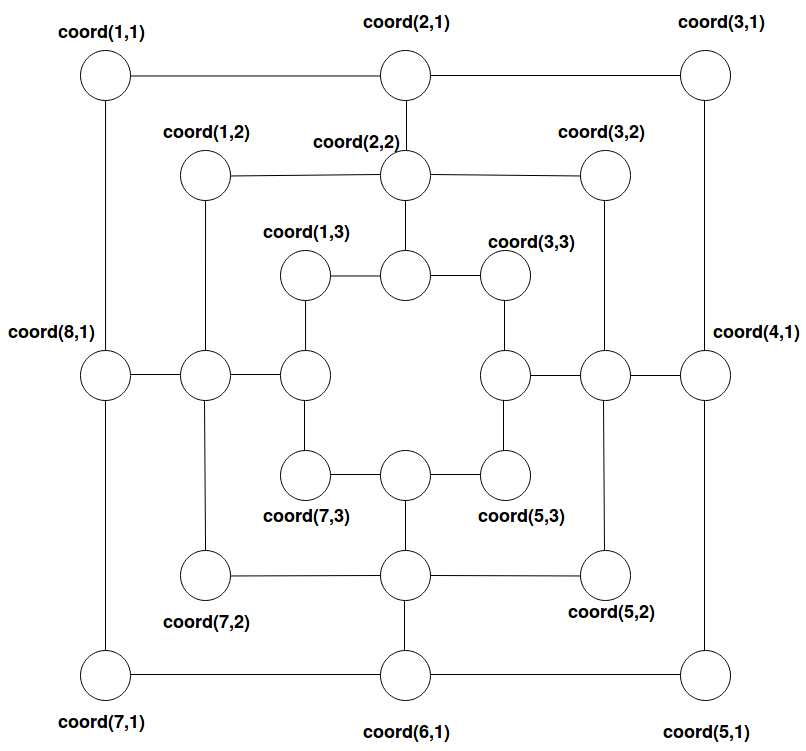
\includegraphics[width = 0.8\hsize]{figures/9MM_coord.png}
\caption{Coordinates of the cells used in Nine Men's Morris}
\label{fig:9MM_coord}
\end{figure}

\subsubsection{Nine Men's Morris described in ASP}

Here, each item refers to the last subsection.

\begin{enumerate}
\item First, we define the players and their roles\\
\texttt{role(player1, red).\\
role(player2, blue).\\}

\item We also add the following rule:\\
\texttt{opponent(P1, P2) :- role(P1, C1), role(P2, C2), P1 != P2.}

\item Here, we describe the game as in \cite{thielscher2009answer}: \texttt{legal/3} only depends on the state of the game (\texttt{holds/2}) and the player that is playing. In other words, we do not take the turn-based aspect into account.

\smallskip

%TODO : Appendix
We will only introduce quickly the predicates that were defined in the ASP Program. You may refer to the complete ASP program (in Appendix ??) for further information. 

%TODO : graph of dependancies.
\begin{tabular}{|c|c|}
\hline 
predicate & description \\ 
\hline
\hline 
\texttt{holds/3} & \makecell{Describes the state of the game: which cells are empty, \\ and which ones contain a pawn of color red or blue.} \\ 
\hline 
\texttt{legal/3} & \makecell{Tells which action a player has the right to perform\\ at a specific time. For instance, \texttt{legal(P,remove\_pawn(C),T)}\\ is true if and only if there is a pawn of the opponent \\in \texttt{C} and this pawn is not in a mill\\ (but if all his pawns form mills, the player \texttt{P} can still remove it)} \\ 
\hline 
\texttt{adjacent/2} & \makecell{Two pairs of coordinates are adjacent if there is an \\ edge that links them (Figure \ref{fig:9MM_coord})} \\ 
\hline 
\texttt{is\_in\_mill/2} & \makecell{\texttt{is\_in\_mill(Coord,mill(Coord\_1, Coord\_2, Coord\_3),T)} \\is true if a player owns the mill \texttt{mill(Coord\_1, Coord\_2, Coord\_3)} \\ and if \texttt{Coord} is one of its three coordinates} \\ 
\hline 
\texttt{has\_mill/3} & \makecell{\texttt{has\_mill(P,Mill,T)} is true if Mill is a mill owned \\by P at time T. It helps to define \texttt{is\_in\_mill/2}} \\ 
\hline 
\texttt{all\_in\_mill/2} & \makecell{Tells if a player has all his pawns in mills} \\ 
\hline 
\texttt{terminal/1} & \makecell{Represents the end of the game (when a player has won).\\ Its only argument is the time \texttt{T}.} \\ 
\hline 
\texttt{wins/2} & \makecell{Tells which player has won and when. \\ A player wins if the other has 2 or less pawns on the board\\ or if the other player is not able to perform any move.}  \\ 
\hline 
\texttt{pawns\_on\_board/3} & \makecell{Counts the number of pawns for each player on the board \\at each time. }\\ 
\hline 
\texttt{able\_to\_play/2} & \makecell{Tells if a player is able to perform any action at a specific time.} \\ 
\hline 
\end{tabular} 

\item After having defined \texttt{legal/3} in the previous step, we add:
\begin{itemize}
\item \texttt{can\_play(Player, place\_pawn, T)} in the body of \texttt{legal(Player, \\place\_pawn(Coord), T) }
\item \texttt{can\_play(Player, move, T)} in the body of \texttt{legal(Player, move(Coord\_1, Coord\_2), T) }
\item \texttt{can\_play(Player, remove\_pawn, T)} in the body of \texttt{legal(Player, \\remove\_pawn(Coord), T) }
\end{itemize}

\item 
We will consider that there are two phases in this game. In the first phase, the players place their respective pawns on the board. And in the second, they have finished to place their pawns and they only move them. 

\bigskip

We suppose that \texttt{player1} starts:
\texttt{can\_play(player1, place\_pawn, 1).} 

\bigskip

To define \texttt{can\_play/3} at time \texttt{T+1} we need to have a closer look at the rules of the game:

\begin{itemize}
\item A player can remove a pawn  at time \texttt{T} if he created a new mill with his action at time \texttt{T-1} (in both phases):\\
\texttt{can\_play(P1, remove\_pawn, T+1) :- does(P1, Action, T), time(T), has\_new\_mill(P1, T+1), role(P1, C1),  phase(phase(1..2),T+1).}
\item Thus, a player can place a pawn if his opponent did not get a new mill with his last action, and if the game is in its first phase:\\
\texttt{can\_play(P1, place\_pawn, T+1) :- does(P2, Action, T), time(T), not has\_new\_mill(P2, T+1), opponent\_player(P1, P2), phase(phase(1),T+1).}
\item Also, a player can move a pawn at time \texttt{T+1} if his opponent did not get a new mill at the same time, and if the game is in its second phase:\\ 
\texttt{can\_play(P1, move, T+1) :- does(P2, Action, T), time(T), \\not has\_new\_mill(P2, T+1), opponent\_player(P1, P2), phase(phase(2),T+1).}
\end{itemize}

The definition of \texttt{has\_new\_meal/2} can be found in appendix ??

\item As there are more than one phase, we add the following definition of \texttt{phase/2} in the program (as explained in the last subsection):\\
\texttt{phase(phase(1), 1).}\\
\texttt{phase(phase(N), T+1) :- time(T), phase(phase(N), T),\\ not finished(phase(N), T+1).}\\
\texttt{phase(phase(N+1), T) :- time(T), finished(phase(N),T).}

\item Finally we define the predicate \texttt{finished/2}:
\begin{itemize}
\item The first phase is finished when both players do not have any pawn in their hands: \\
\texttt{finished(phase(1), T) :- time(T), has\_pawns(player1, 0, T), \\has\_pawns(player2, 0, T).}\\
Where \texttt{has\_pawns/3} counts the number of pawns that each player still has to place. Its complete definition may be found in appendix ??
%TODO : faire une recherche sur le latex pour les ?? et les remplacer
\item We suppose that the second phase never finishes (as there is no third phase). So we do not need to define \texttt{finished(phase(2), T)}. 
\end{itemize}

\end{enumerate}